\clearpage



\appendix{} 

\vskip -0.3in
\leftline{\bf A. Fitting the mixture model}
\label{app:v12-fitting}

We fit the V12 model in stages. In a given band, let $x=\Delta m=m_{\rm PSF}-m_{\rm S\acute{e}rsic}$ and let $m$ be the S\'{e}rsic magnitude in that band. At a given magnitude, we describe the distribution of $x$ as a mixture of unresolved (U) and resolved (R) components:
\begin{equation}
 p(x\mid m)=w_U(m)U(x\mid m)+[1-w_U(m)]R(x\mid m).
\end{equation}
The functions $U$ and $R$ describe the component shapes, and $w_U$ is the fraction assigned to U. The component densities are normalized on $W=(-0.5,1.5)$ mag. Figure~\ref{fig:v12-fitting-steps} illustrates the stages for the $r$ band. These are model components, not HST class histograms.

\noindent\textbf{Parent-sample fit.} We first fit Rubin parent photometry without using external class labels. The U component is a narrow Johnson $S_U$ distribution; the R component is a mixture of two skew-normal distributions. Their shapes and relative proportions are fitted to the observed $\Delta m$ distribution. We then keep the fitted U shape and parent U/R fraction fixed while refining the R distribution as a continuous function of magnitude. The U peak center $\mu_c(m)$ and its local curvature width $\sigma_c(m)$ provide the narrow-core reference for $D$ and are retained in the subsequent fits.

\noindent\textbf{Reference-sample fraction.} We next use Rubin photometry for the cleaned HST-associated reference cohort. Keeping the parent U and R shapes fixed, we fit the U fraction
\begin{equation}
 w_U(m)=w_{\rm floor}+(1-w_{\rm floor})[1+\exp\{-c-d(m-22)\}]^{-1}.
\end{equation}
The fitted fraction is conditional on the parent shapes. In the $r$-band example at $m=24.5$, the U fraction changes from approximately 2.8\% in the parent model to 3.2\% after reference-sample calibration.

\noindent\textbf{Reference-sample shapes.} Keeping the narrow U core and the reference-sample U/R fraction fixed, we add a positive tail to U and refit the R shape:
\begin{equation}
 U(x\mid m)=[1-f(m)]J(x\mid m)+f(m)T(x\mid m),\quad
 f(m)=[1+\exp\{-f_0-f_1(m-22)\}]^{-1}.
\end{equation}
Here $J$ is the retained narrow core, $T$ is a lognormal density in the positive offset $x-\mu_c(m)$, and $f(m)$ is the fraction of U assigned to the tail. Before normalization on $W$, the tail's median offset is $\kappa\sigma_c(m)$ and its logarithmic width is $h$. The tail parameters and the R-shape parameters are fitted together. Adding the tail changes the full U distribution, while the center and local width of the retained core remain fixed. At $m=24.5$, the tail contains approximately 41.6\% of U; this is a fraction within U, not a fraction of all objects. For $r$, the fitted parameters are $(c,d,w_{\rm floor})=(-2.30135,-0.87596,0.02157)$ and $(f_0,f_1,\kappa,h)=(-3.84233,1.40185,14.1174,1.7906)$.

\noindent\textbf{Likelihood and checks.} The reference-sample fraction is fitted using individual objects' photometry. The final U-tail and R-shape fit uses 0.125-mag magnitude cells and 0.004-mag $\Delta m$ bins. Its model probability for each bin is obtained by integrating the density across the bin, rather than evaluating it only at the bin center. We use three starting points and select the largest training likelihood. An object-ID hash supplies training and held-out subsets for a photometric check; the final parameters are then refitted using all eligible objects. In the continuous R and final reference fits, the representative magnitude of each fine cell is calculated using all eligible objects in the cell, including held-out objects; the check is therefore not fully independent of preprocessing.

Reference membership is based on the cleaned HST-associated sample, but HST star/galaxy labels are not used in the numerical fits. Those labels are used afterward for evaluation and method selection. The comparison in Figure~\ref{fig:v12-fitting-steps} shows the fitted distributions on the reference sample and is not an independent blind test.

\begin{figure*}[p]
\centering
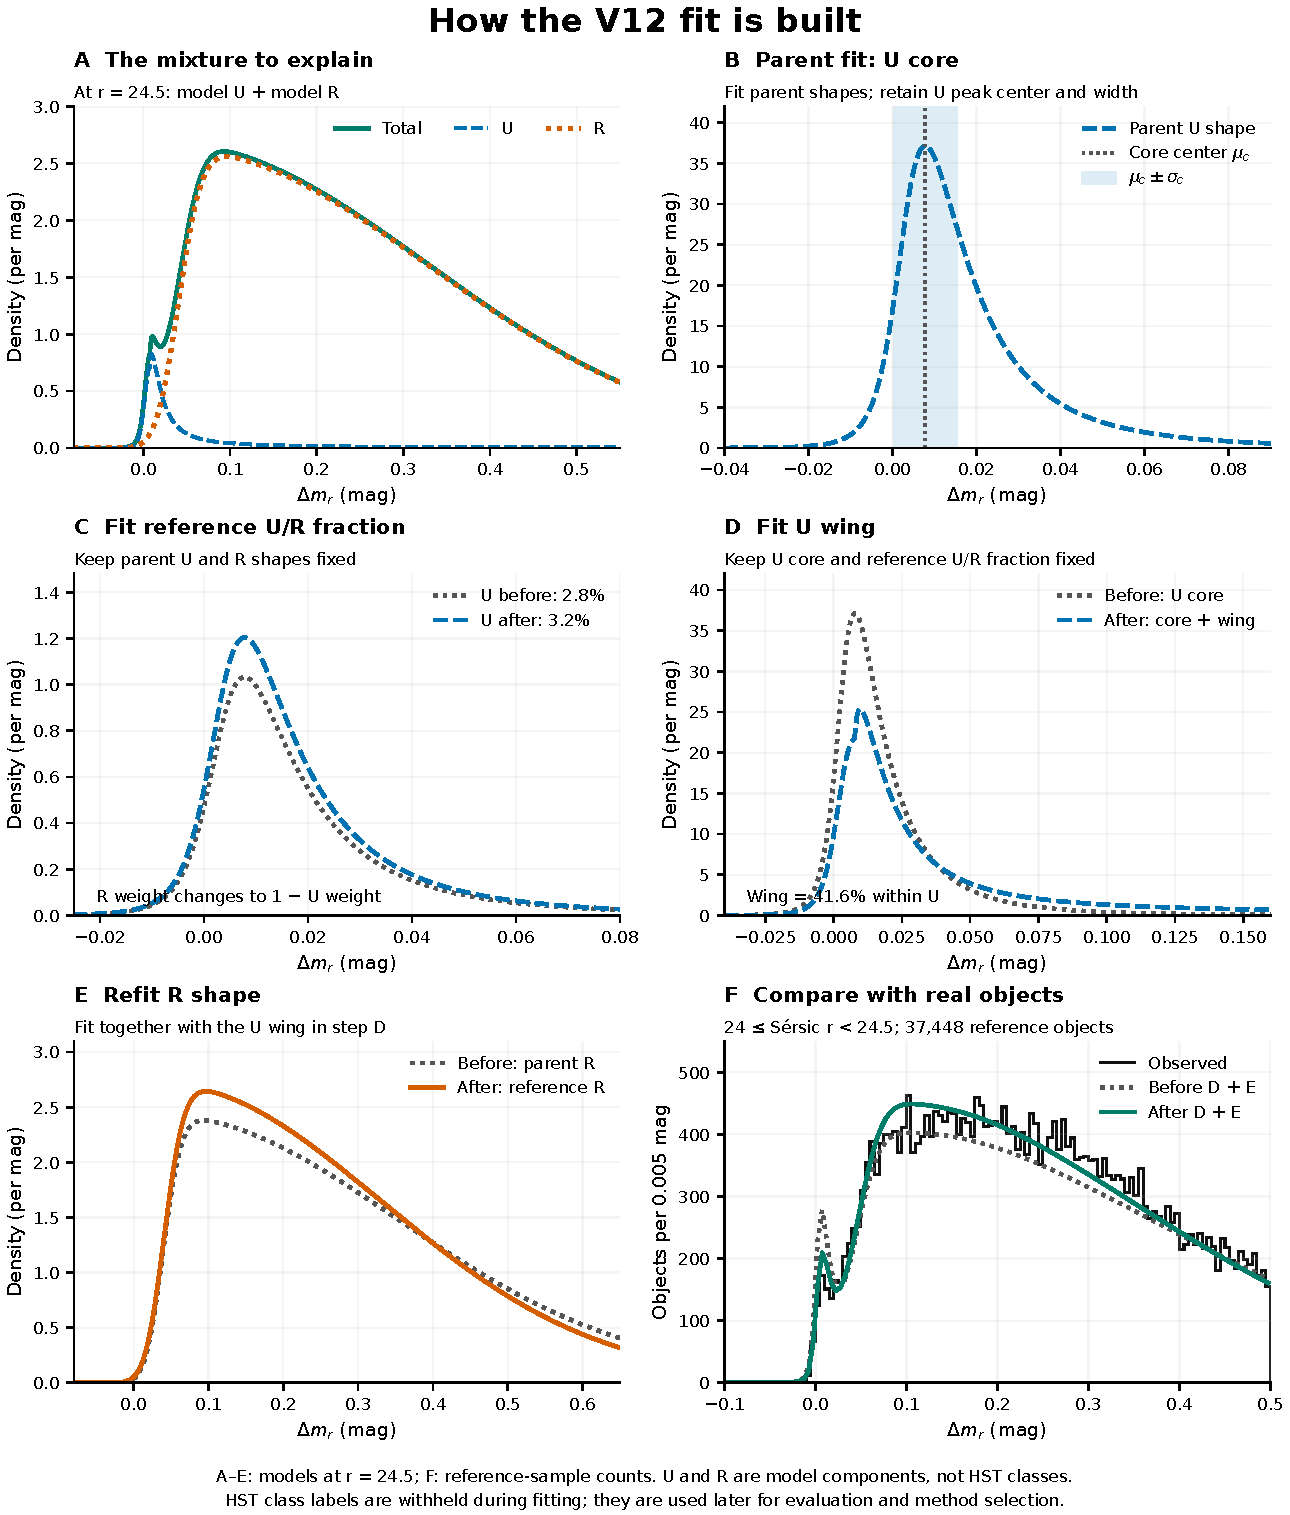
\includegraphics[width=\textwidth,height=0.70\textheight,keepaspectratio]{V12_fitting_one_figure.pdf}
\caption{XXXX}
\label{fig:v12-fitting-steps}
\end{figure*}

\vskip 0.3in
\leftline{\bf B. Reproducing \texttt{griz\_model\_extendedness} parameter} 


Here Daniel describes corrections for uncertainties and size... 


% OLD toy models
%Figures~\ref{fig:toymodel1} and~\ref{fig:toymodel2} illustrate simulated
%unresolved and resolved populations and comparisons with model predictions.

%\begin{figure*}
% \centering
%  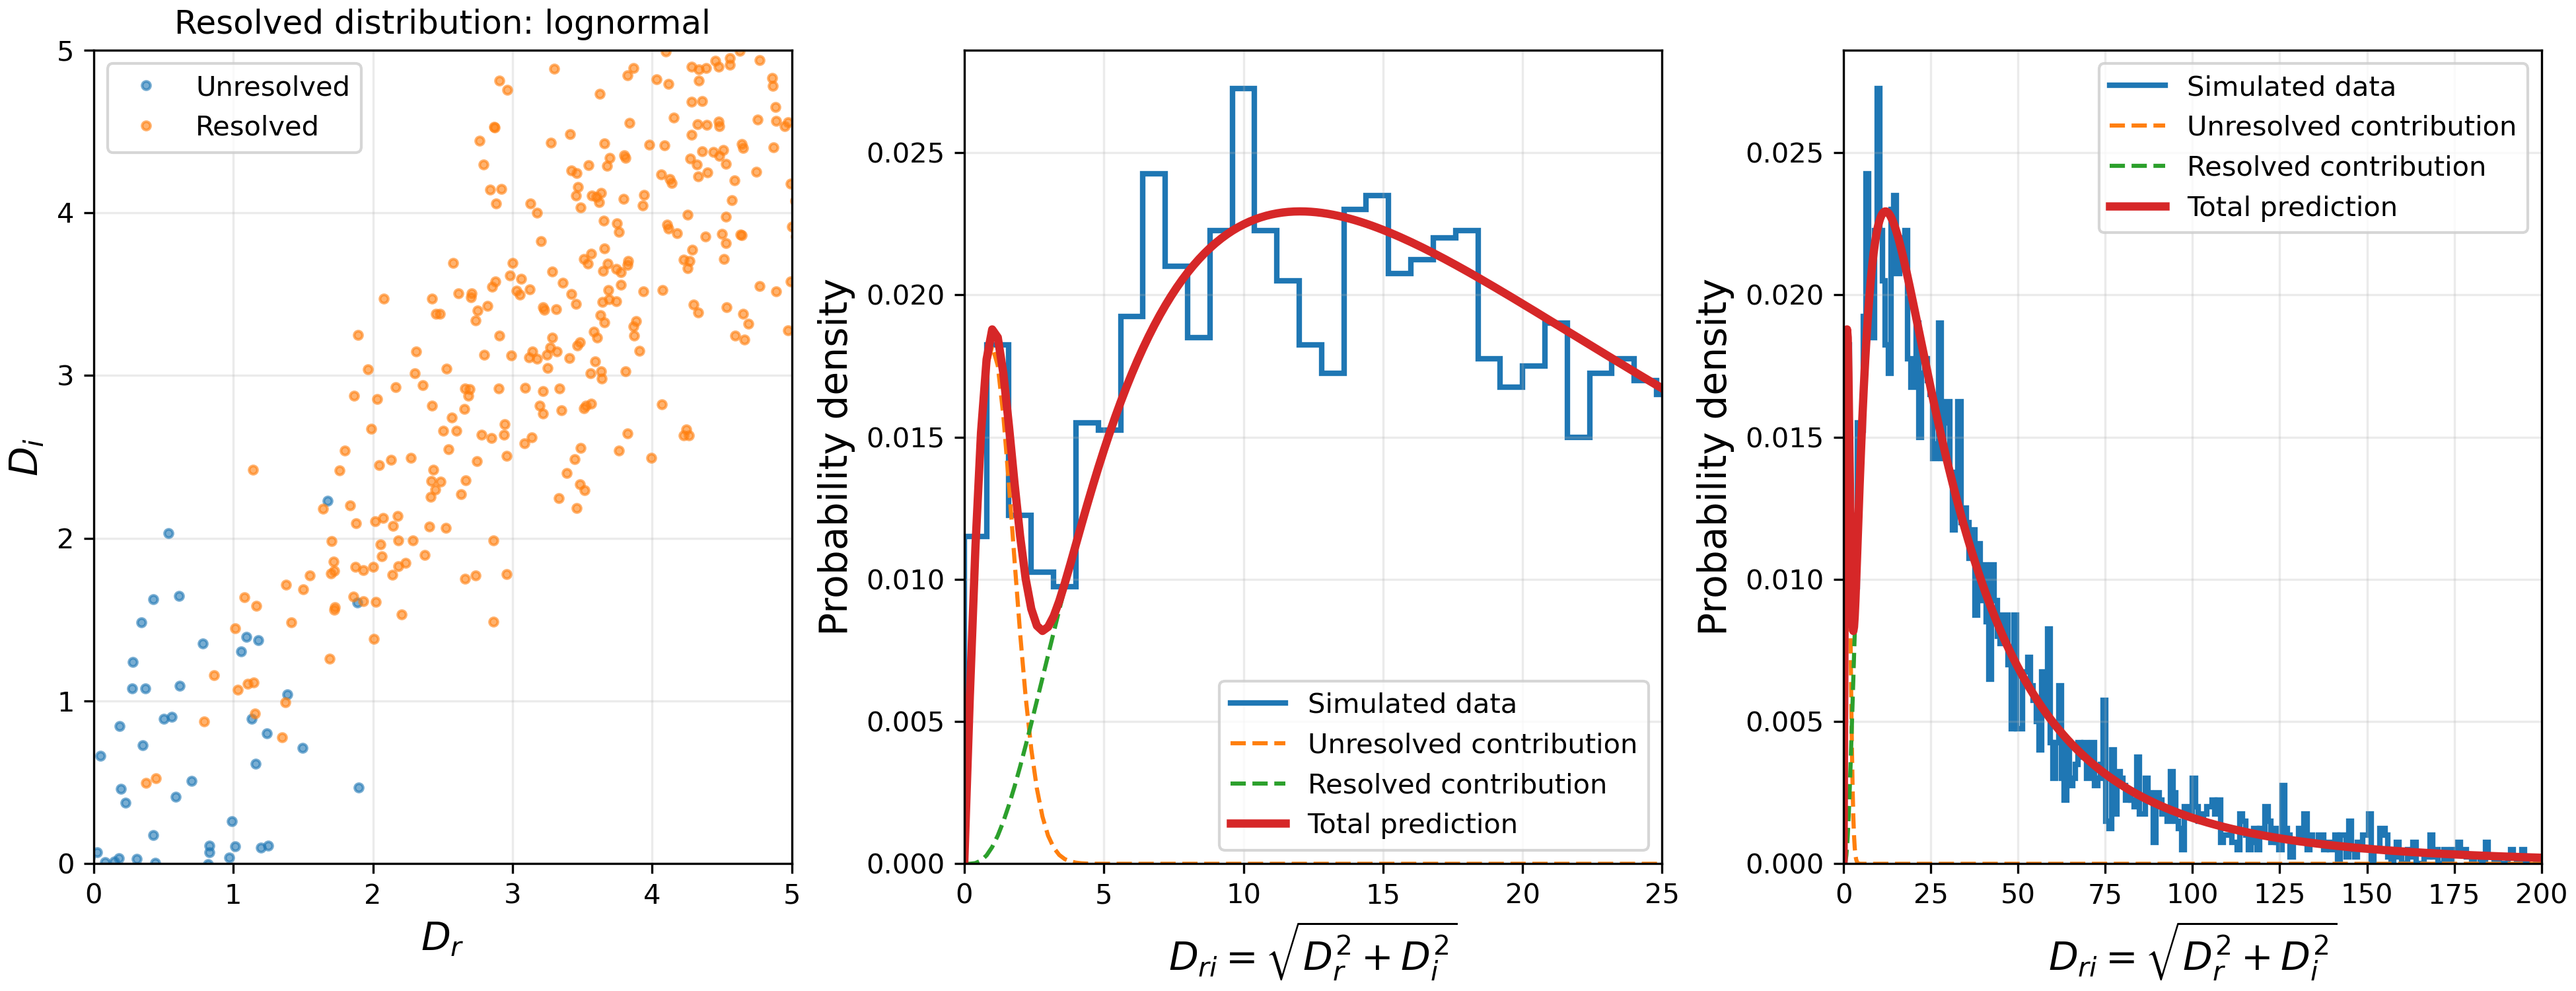
\includegraphics[width=\textwidth]{simulate_and_plot.png}
%  \caption{Illustrative simulated unresolved and resolved populations
%  (left), with comparisons of simulated histograms, component predictions,
%  and total predictions (middle and right).}
%  \label{fig:toymodel1}
%\end{figure*}


%\begin{figure*}
%  \centering
%  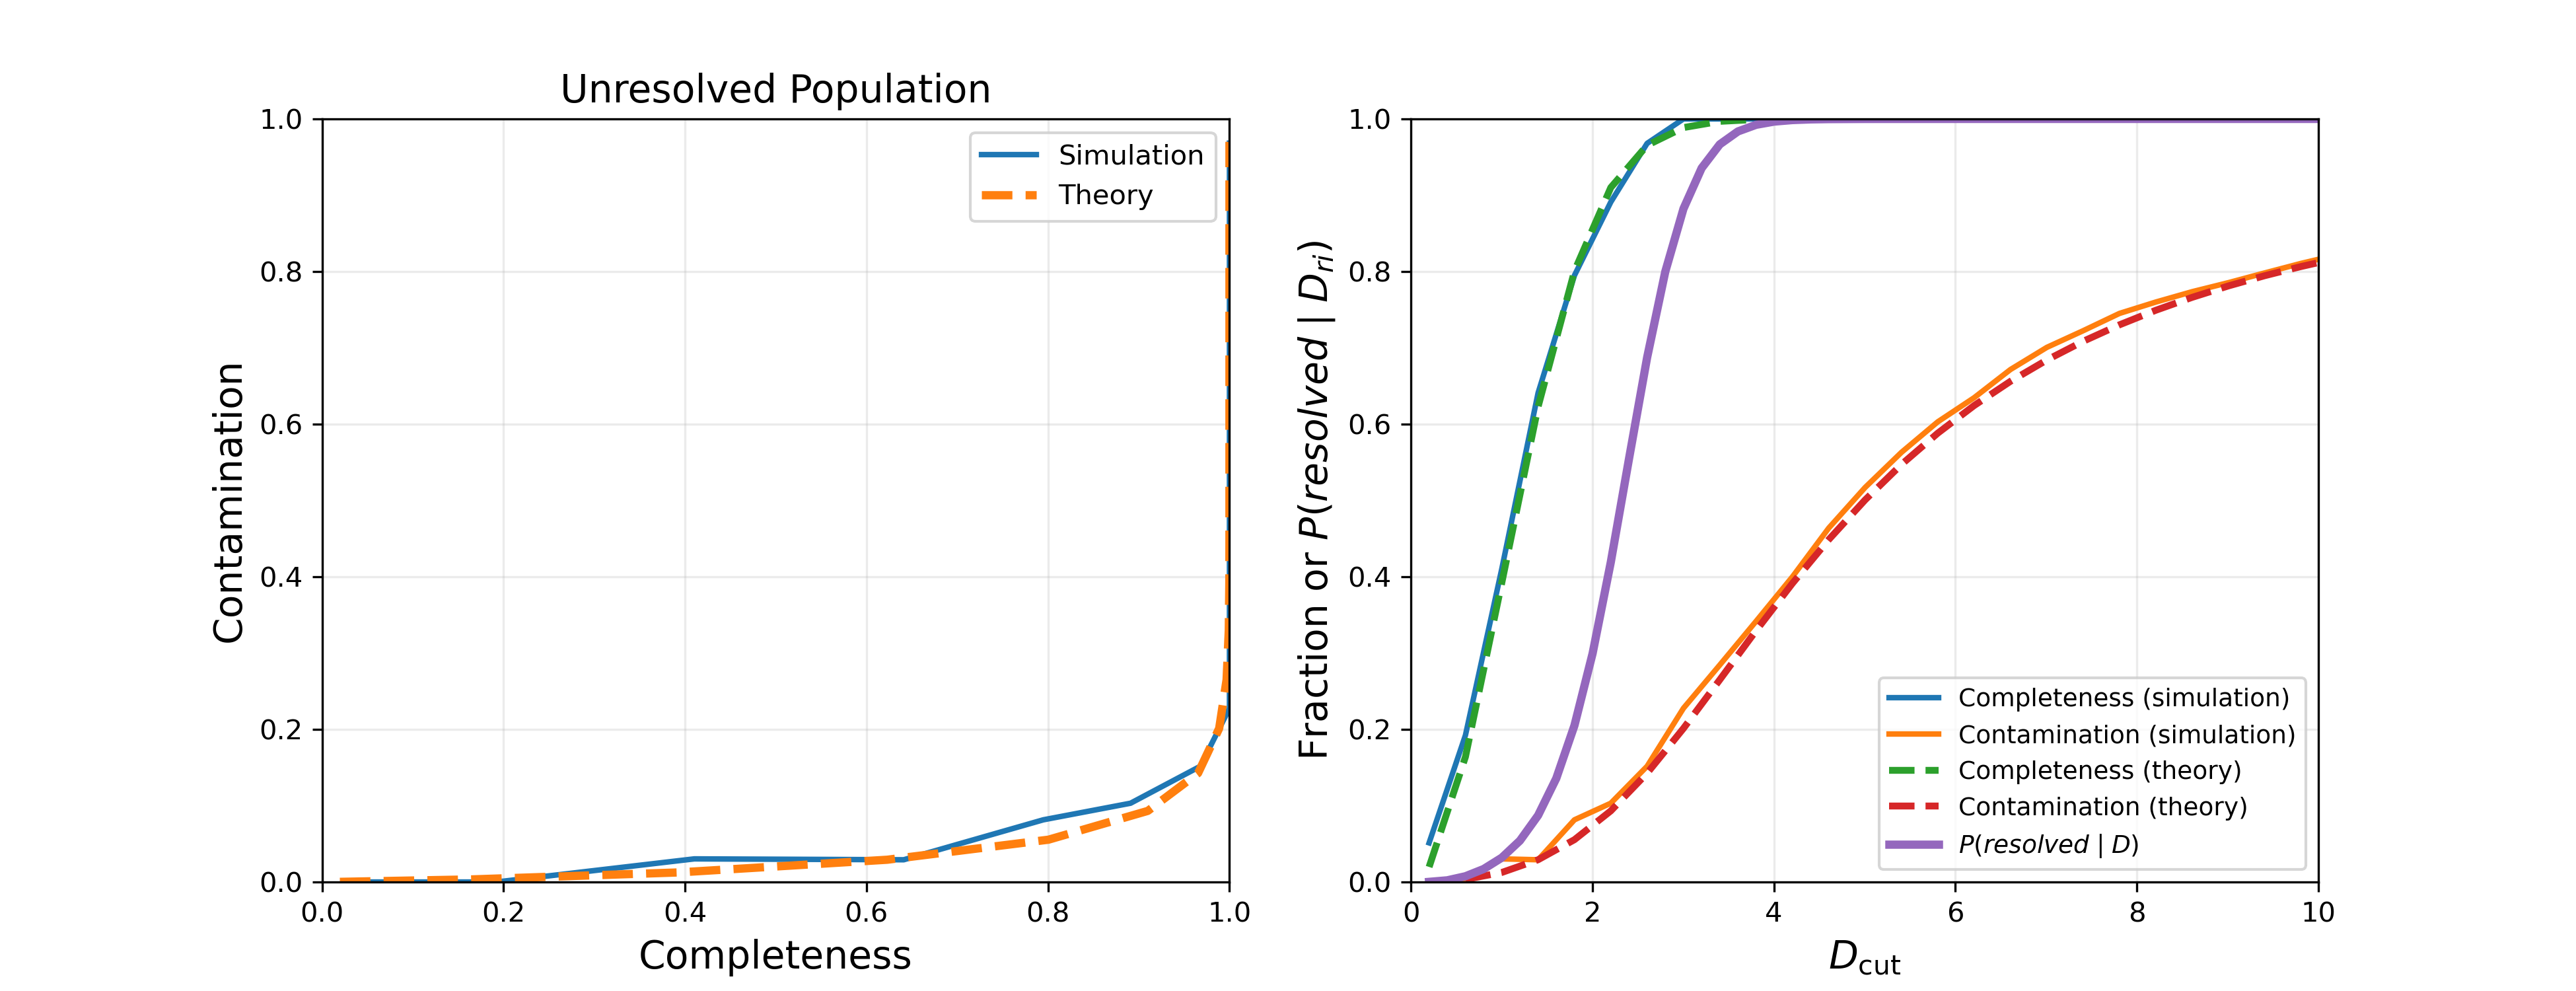
\includegraphics[width=\textwidth]{simulation_vs_theory.png}
%  \caption{Second figure...}
%  \label{fig:toymodel2}
%\end{figure*}

\clearpage
\begin{figure*}[p]
  \centering
  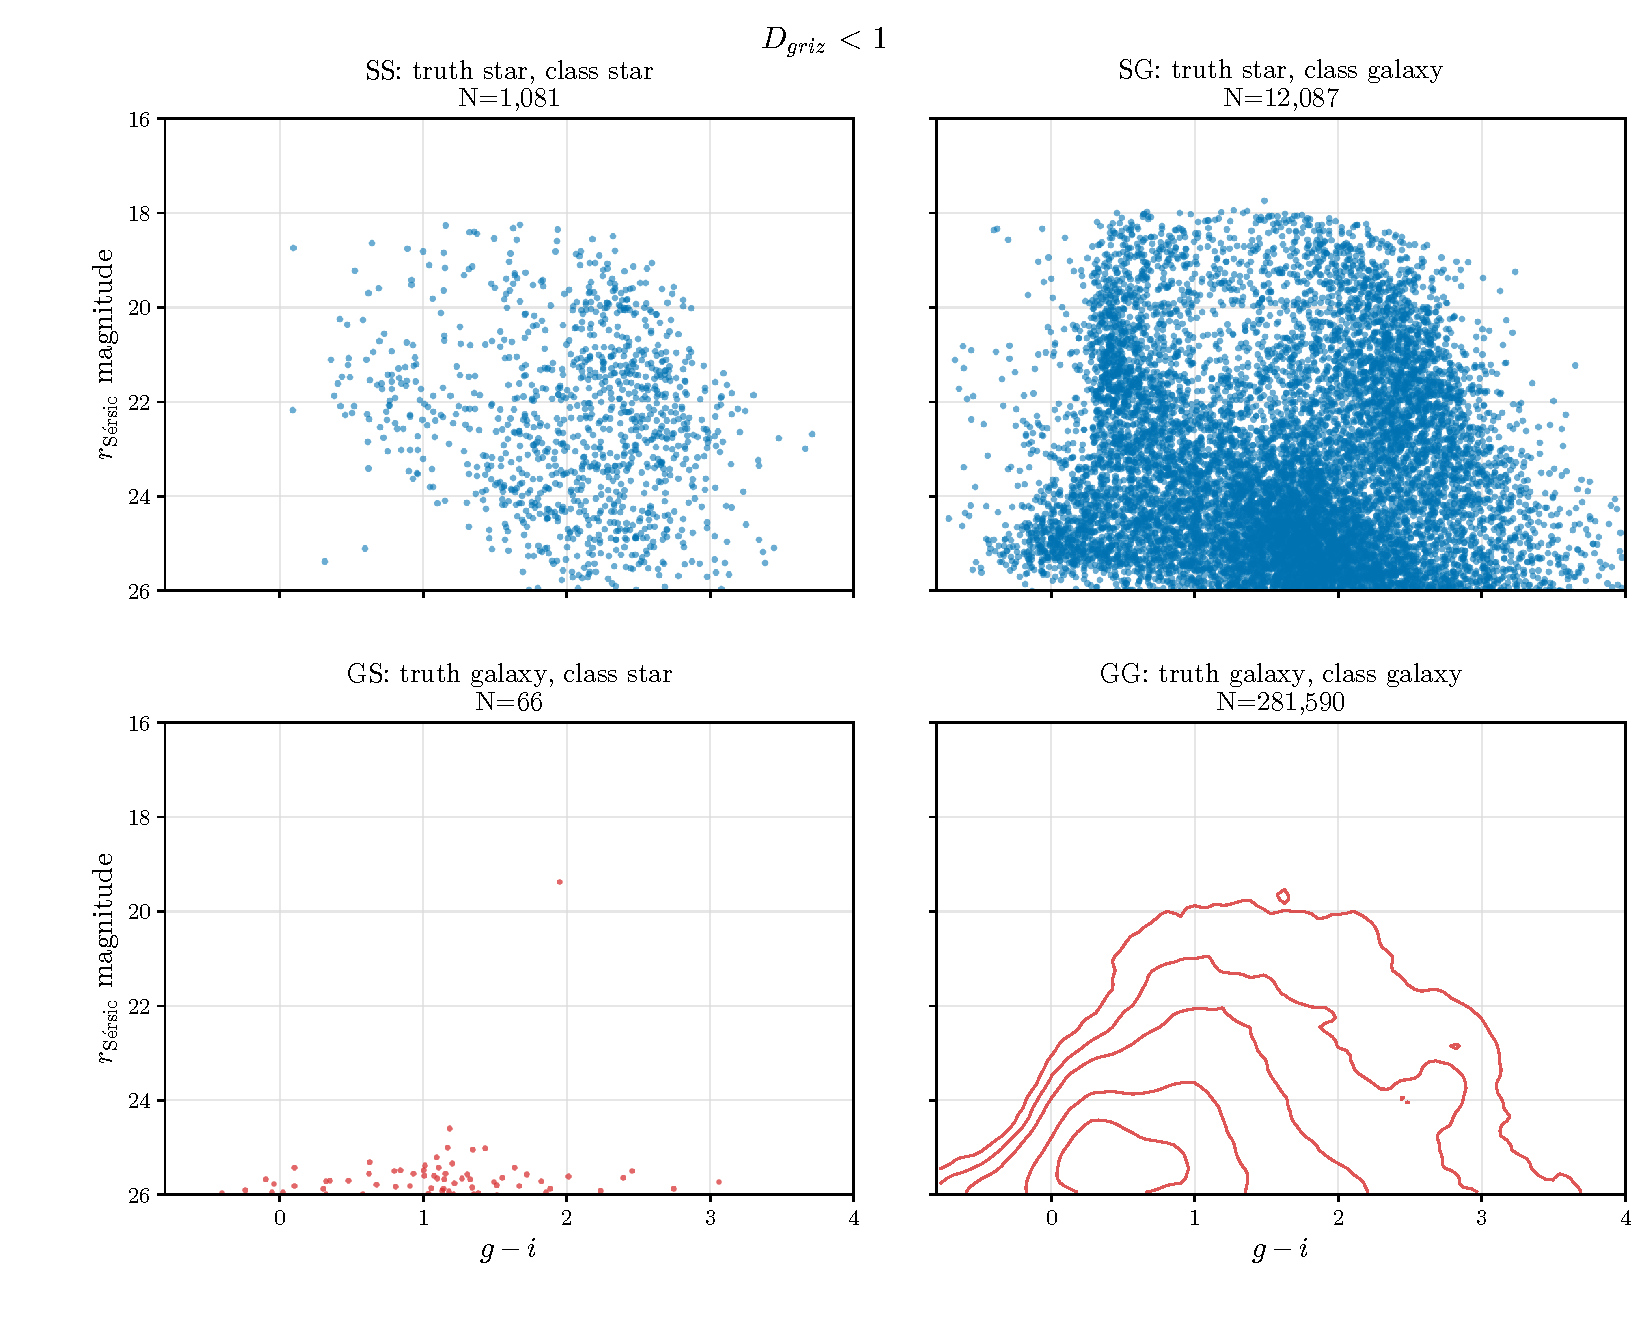
\includegraphics[width=0.9\textwidth,height=0.43\textheight,keepaspectratio]{figures/fixed_completeness_and_comparisons/03_Fig5_Dgriz_1.pdf}
  \caption{}
  \label{fig:appendix-dgriz-cut-1}
\end{figure*}
\begin{figure*}[p]
  \centering
  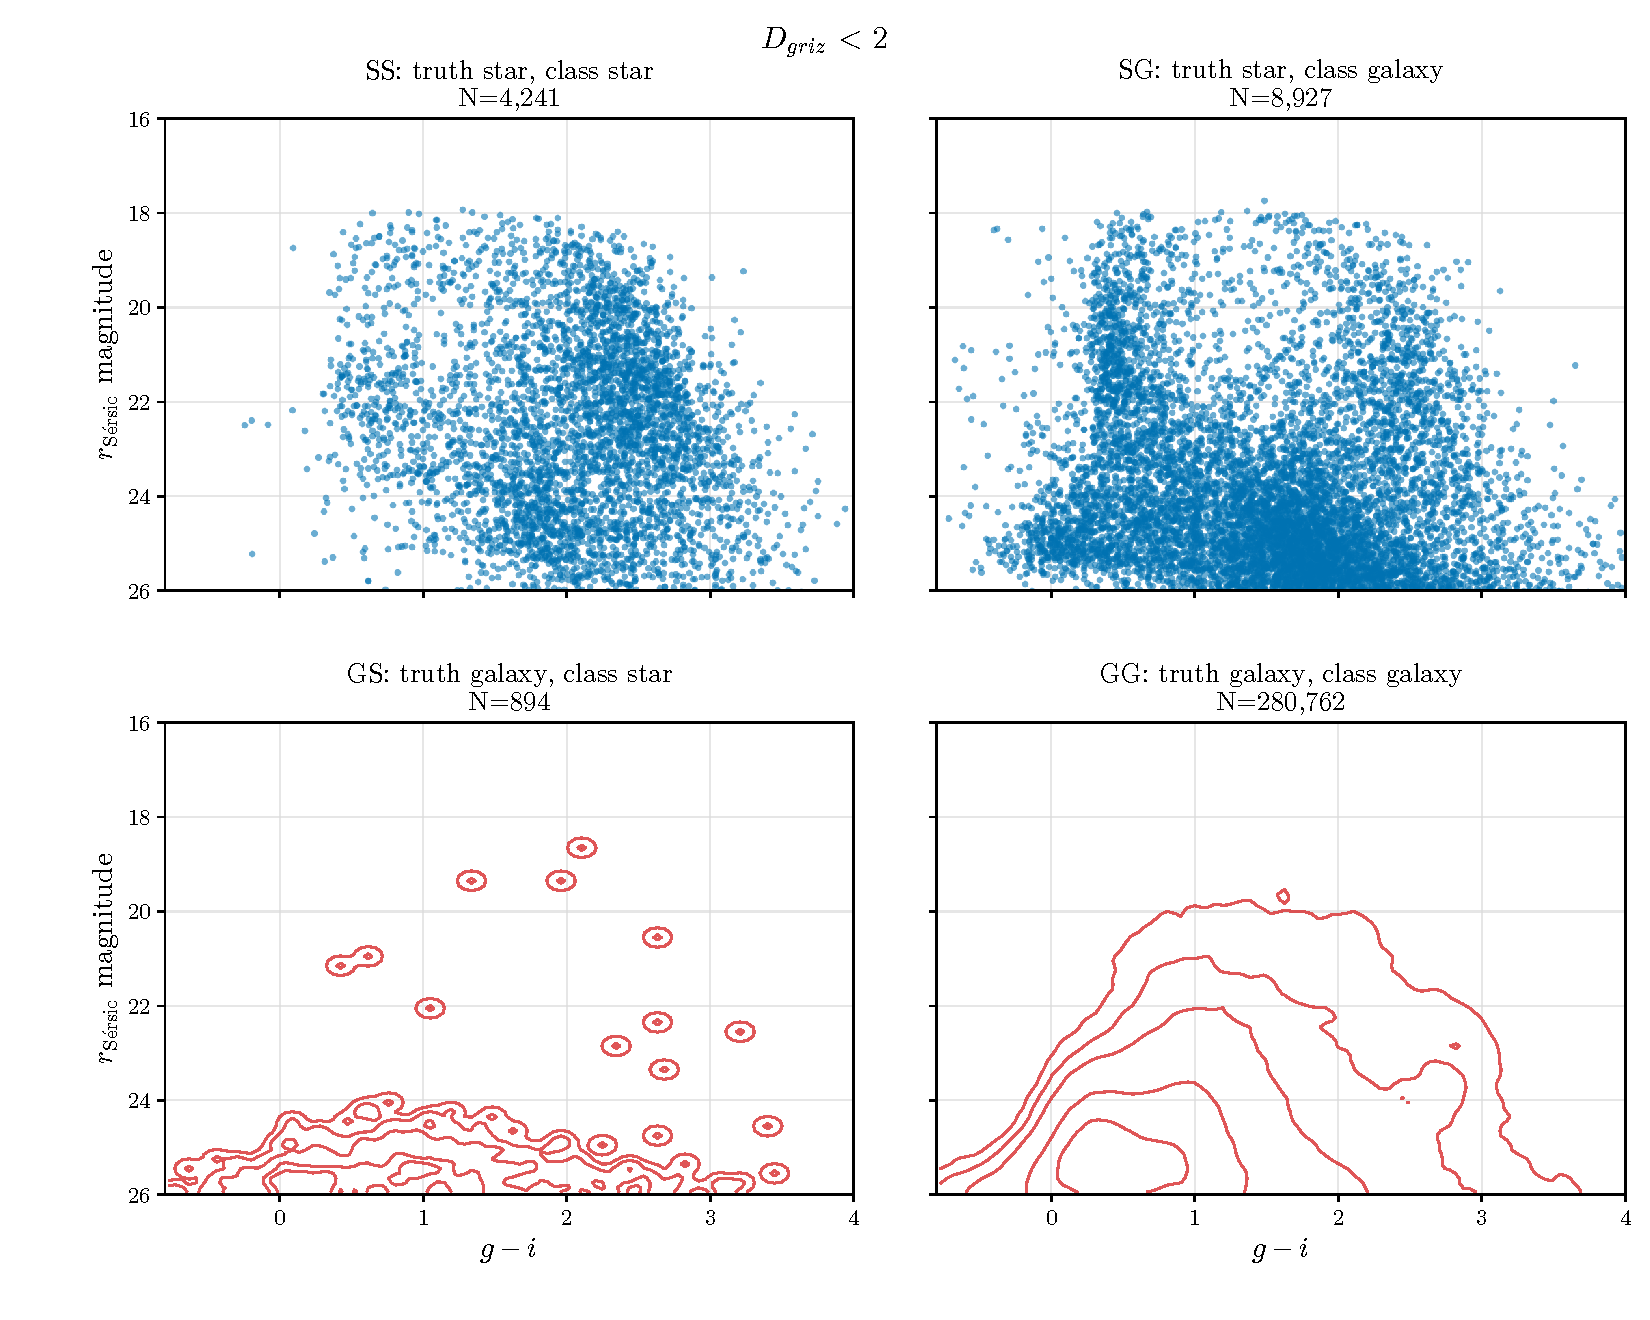
\includegraphics[width=0.9\textwidth,height=0.43\textheight,keepaspectratio]{figures/fixed_completeness_and_comparisons/03_Fig5_Dgriz_2.pdf}
  \caption{}
  \label{fig:appendix-dgriz-cut-2}
\end{figure*}
\begin{figure*}[p]
  \centering
  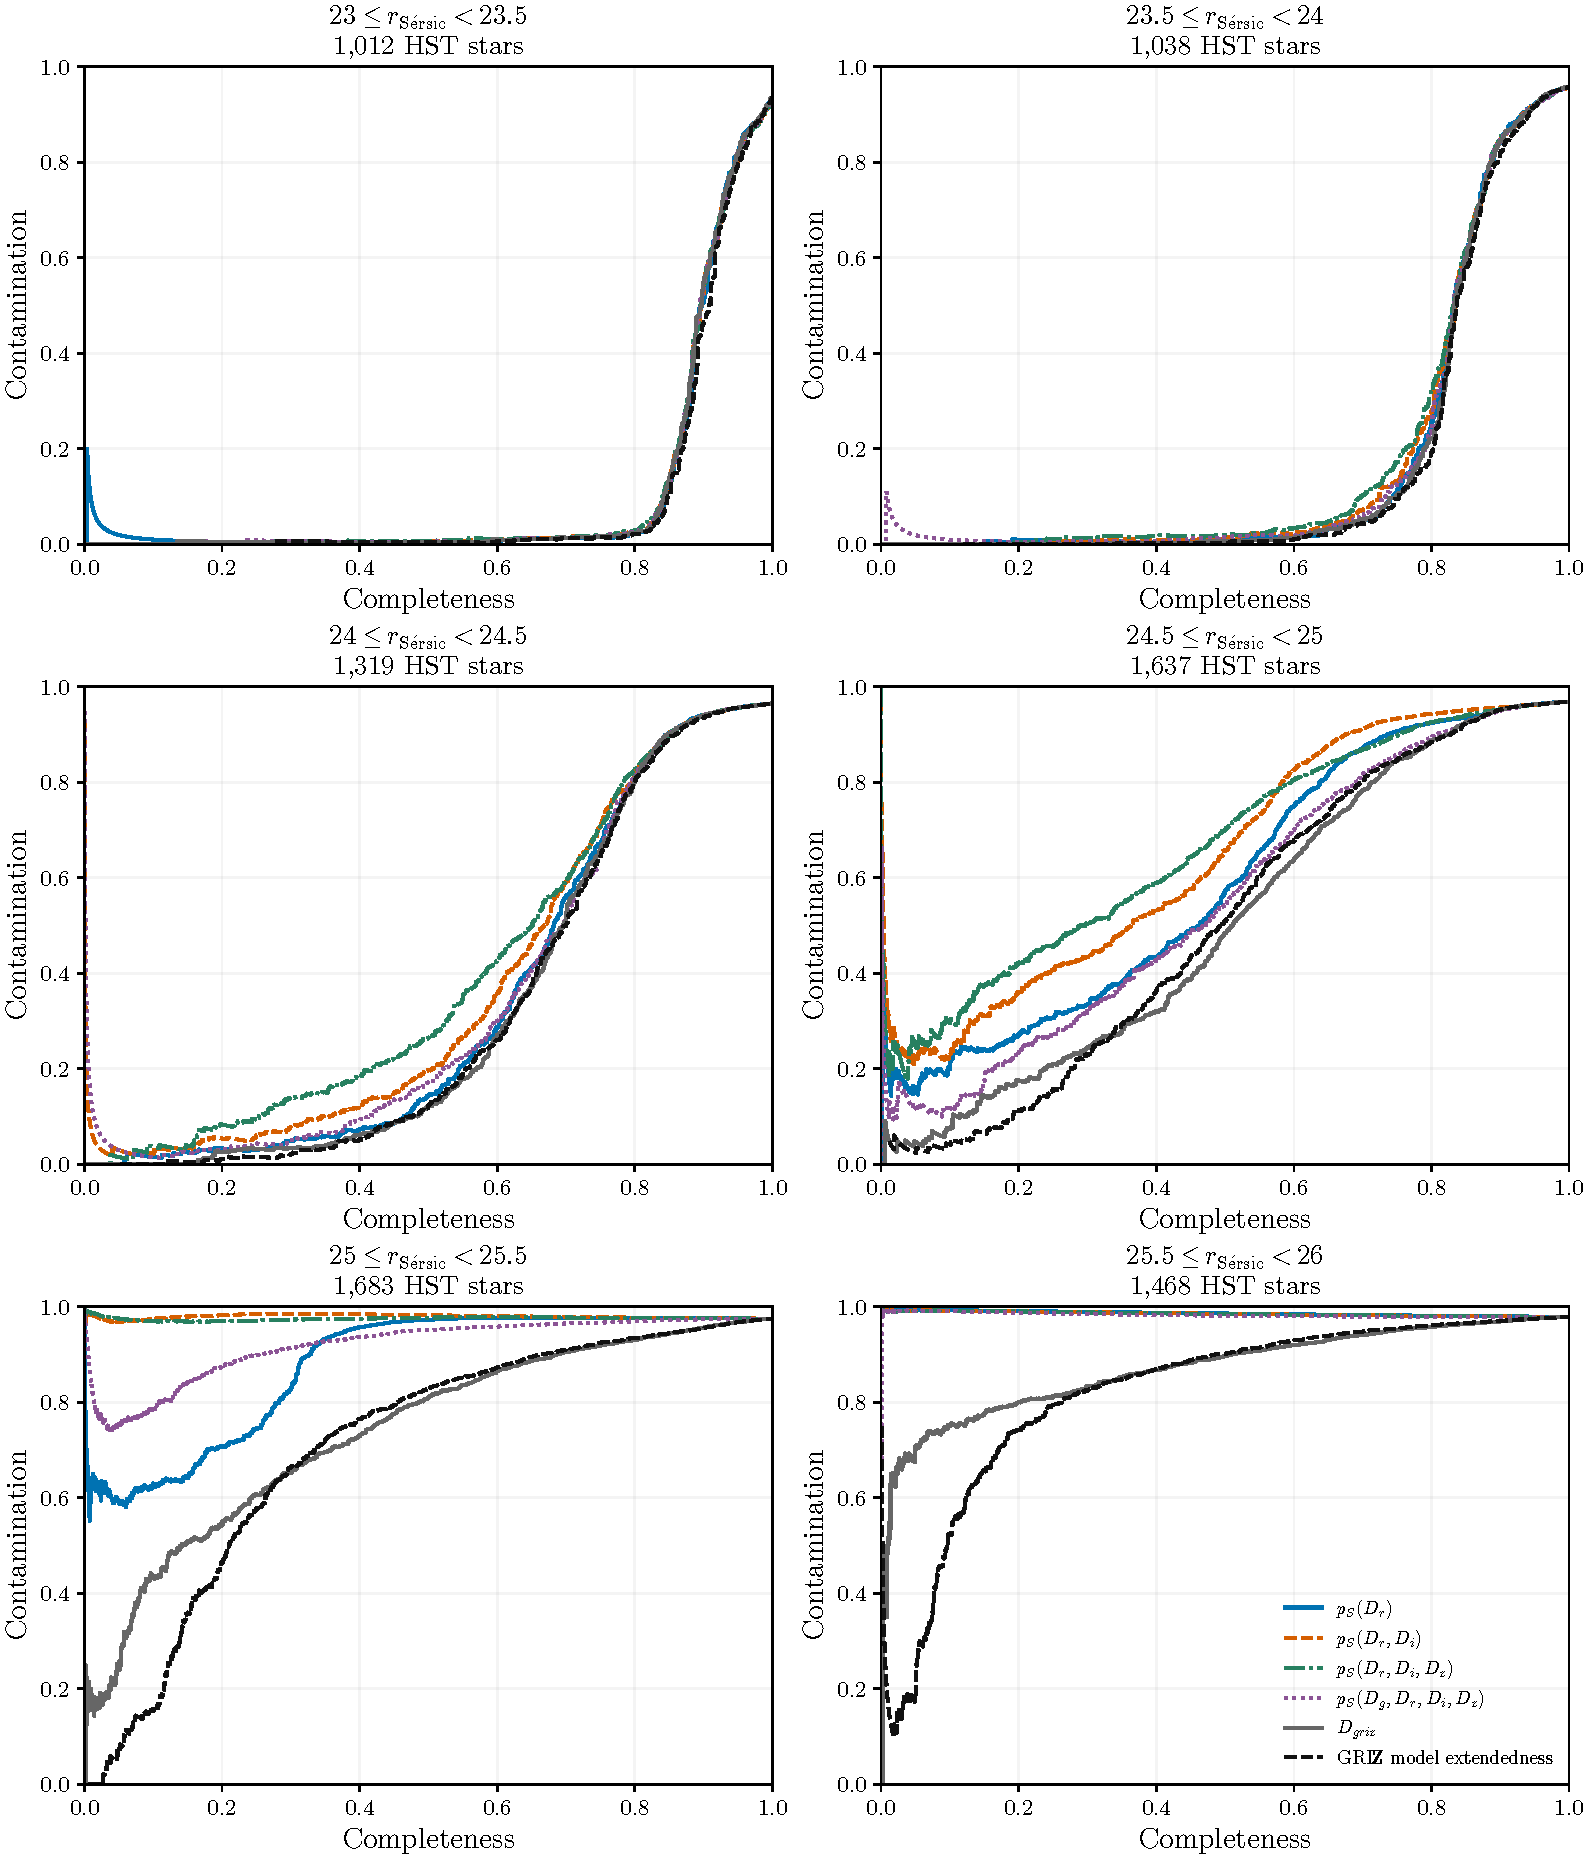
\includegraphics[width=0.9\textwidth,height=0.80\textheight,keepaspectratio]{figures/fixed_completeness_and_comparisons/04_01_Logodds_single_to_multi.pdf}
  \caption{}
  \label{fig:appendix-logodds-bands}
\end{figure*}
\begin{figure*}[p]
  \centering
  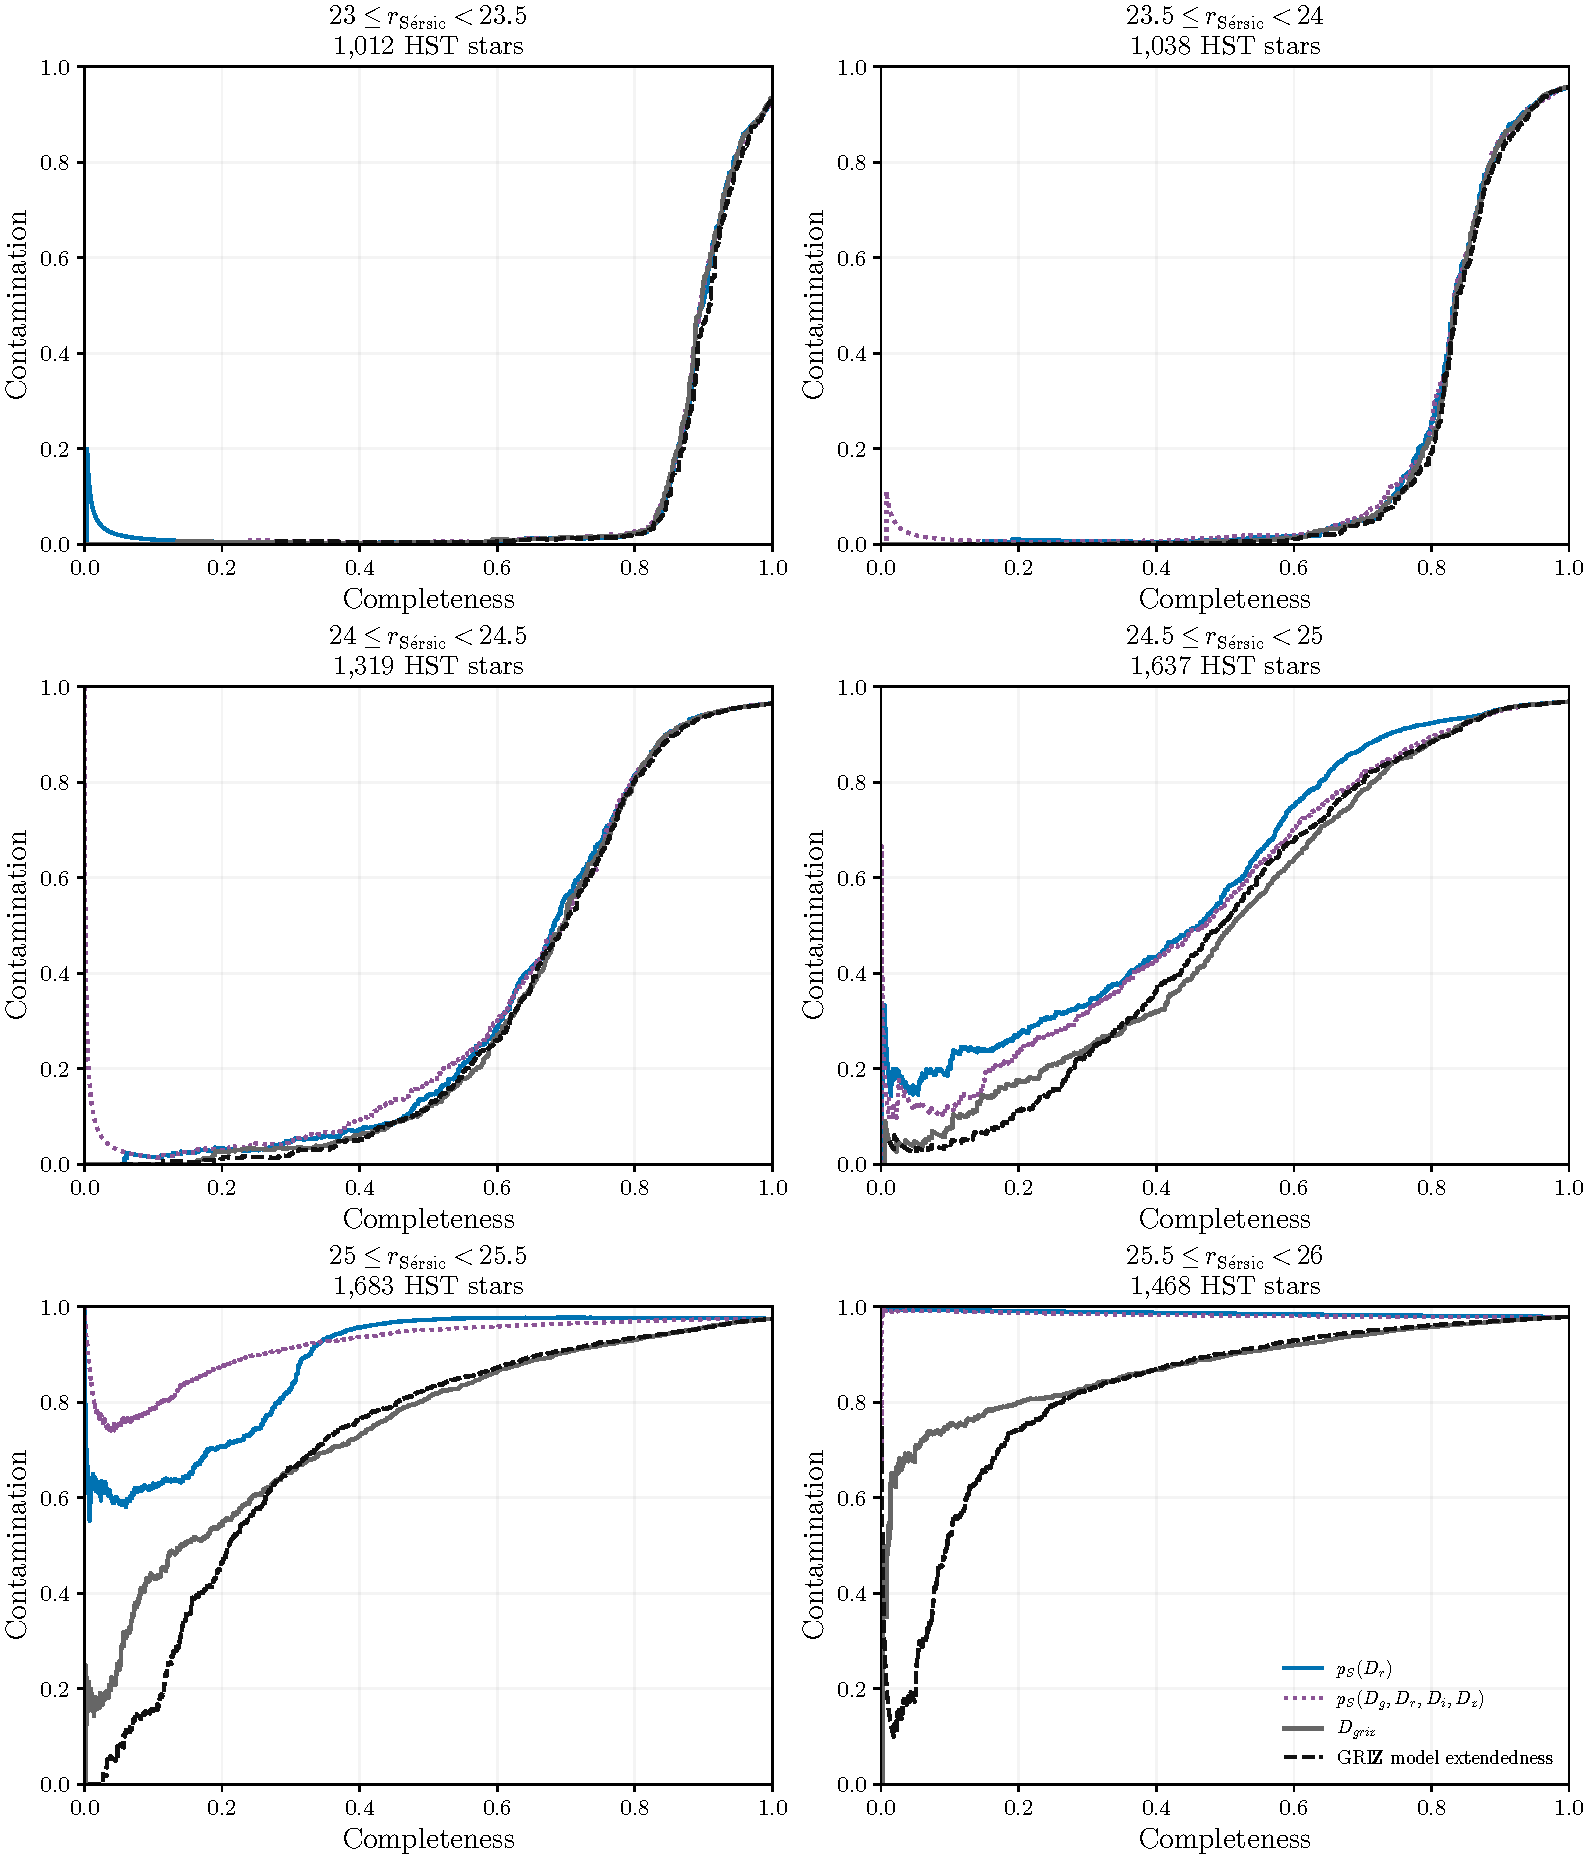
\includegraphics[width=0.9\textwidth,height=0.80\textheight,keepaspectratio]{figures/fixed_completeness_and_comparisons/04_02_Logodds_vs_original_D_and_extendedness.pdf}
  \caption{}
  \label{fig:appendix-logodds-comparison}
\end{figure*}
\begin{figure*}[p]
  \centering
  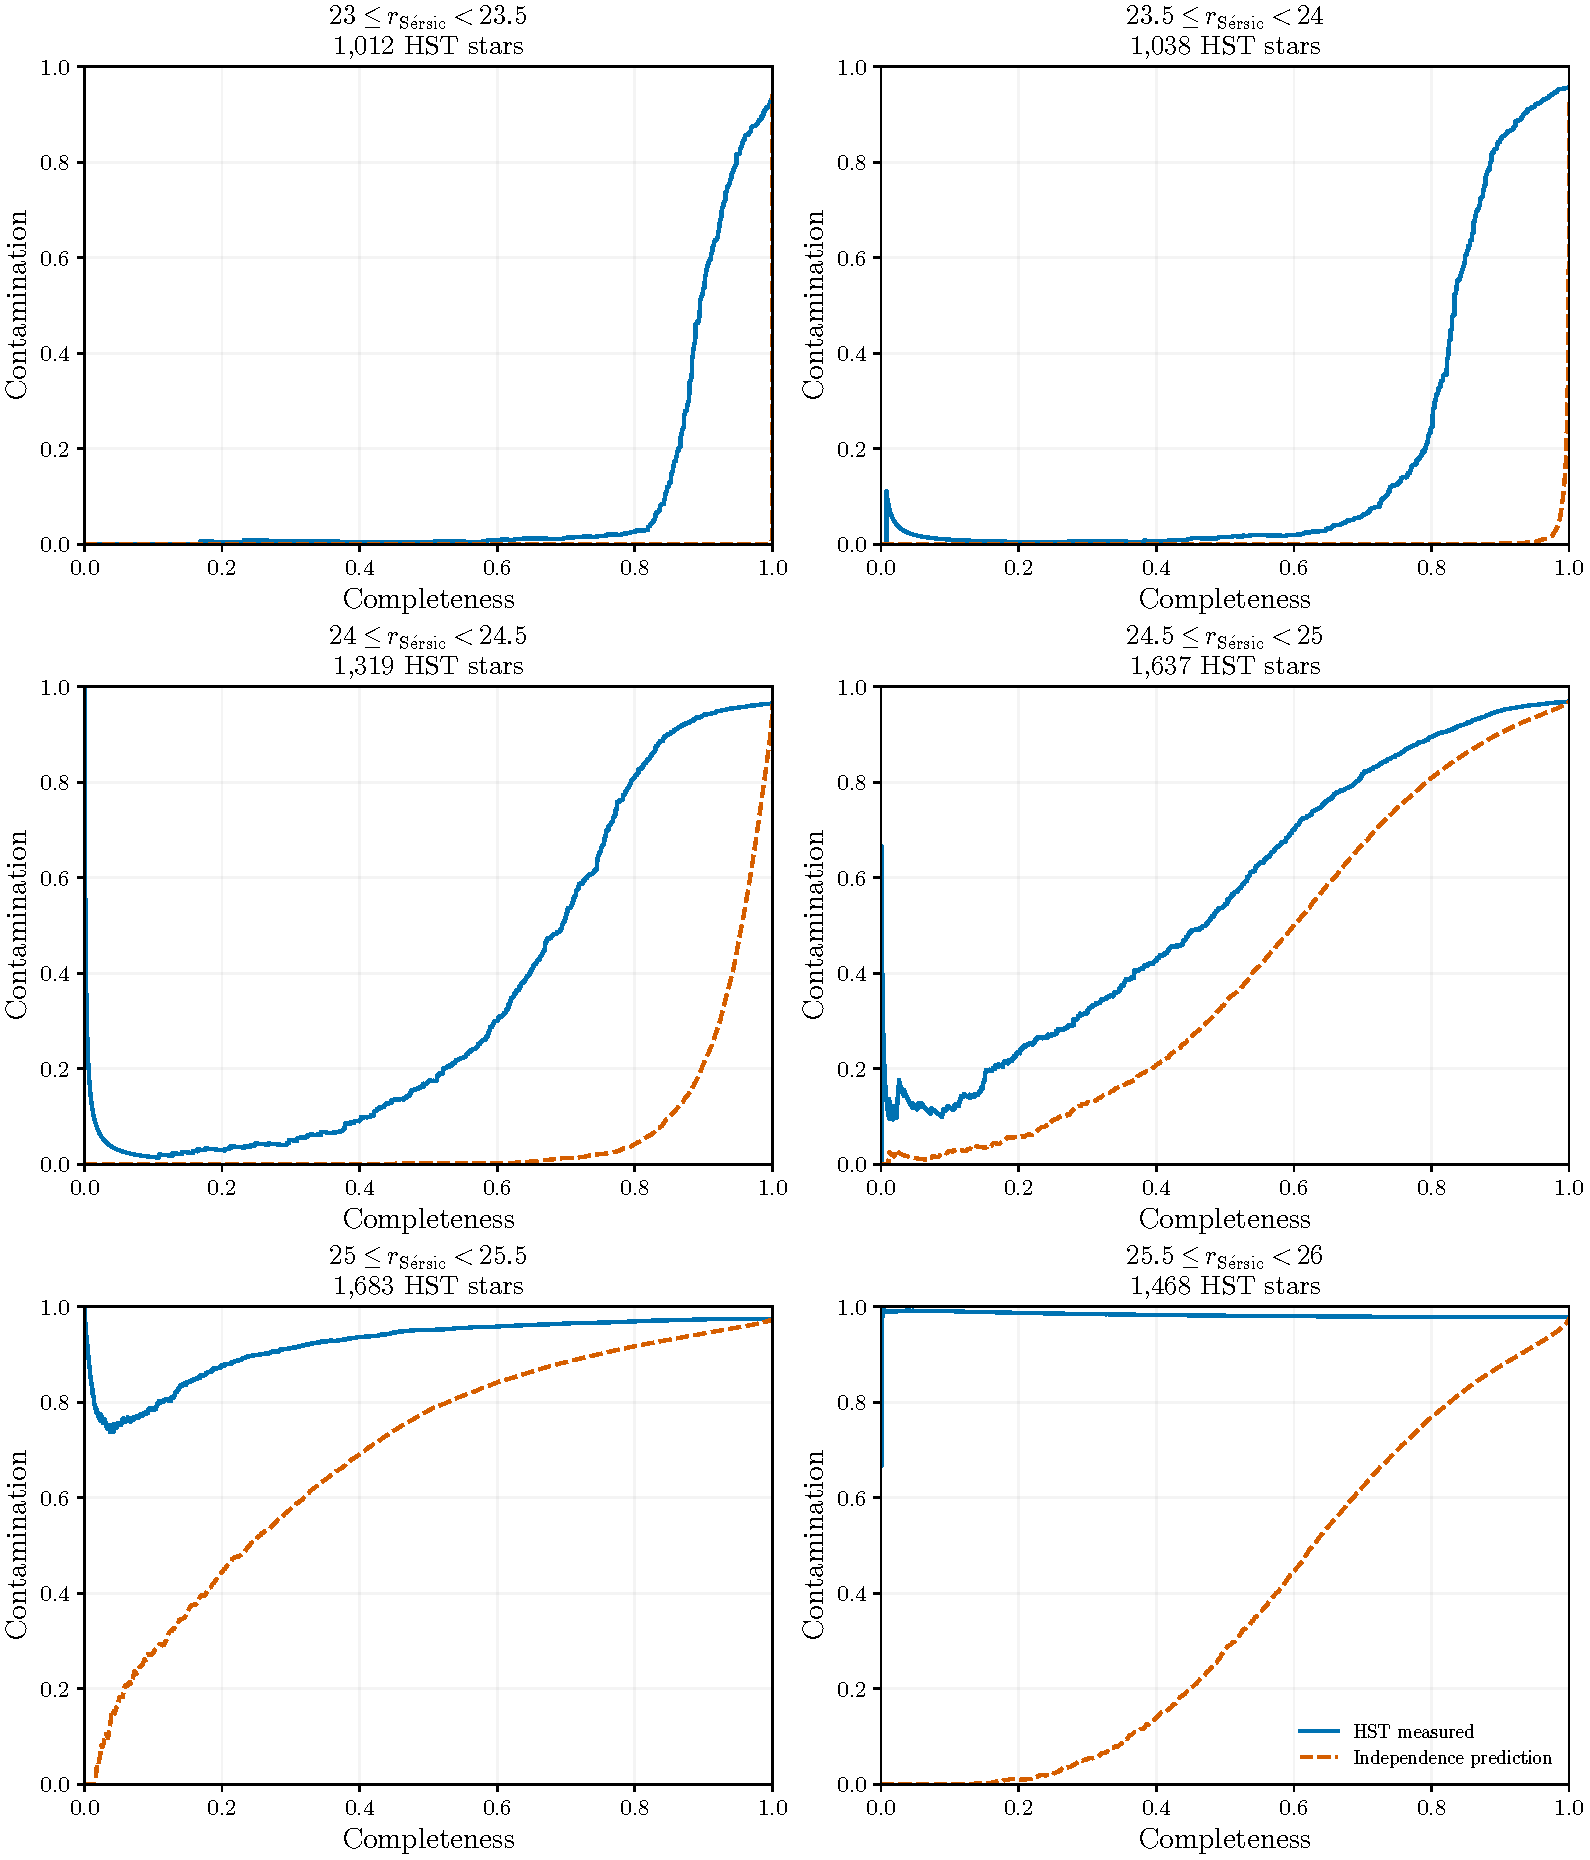
\includegraphics[width=0.9\textwidth,height=0.80\textheight,keepaspectratio]{figures/fixed_completeness_and_comparisons/04_03_Logodds_predicted_CC_vs_HST.pdf}
  \caption{}
  \label{fig:appendix-logodds-prediction}
\end{figure*}
\clearpage
